\documentclass{article}
\usepackage{amsmath}
\usepackage{amsfonts}
\usepackage{amssymb}
\usepackage{courier}
\usepackage{graphicx}
\usepackage{subfig}
\usepackage{listings}
\usepackage[margin=1in]{geometry}

\title{Stock Market Predictor using Backpropagation Neural Networks}
\begin{document}
\nocite{*}


\begin{titlepage}
    \begin{center}
        \vspace*{7.5cm}
        {\bf Stock Market Predictor using Backpropagation Neural Networks}
        
        \vspace{0.5cm}
        
        \vspace{7.5cm}        
        
        \textbf{David Leonard}
	
	\vspace{0.5cm} 
	Date: May 2, 2016
        
        \vspace{1in}
        \vfill
        
    \end{center}
\end{titlepage}

\tableofcontents

\newpage

\section{Introduction}

One of the biggest fields in the financial sector is machine learning - understanding how to properly build algorithms which can self-learn and have a certain degree of predictive power over the trends of the stock market. While conspiracies and theories have stated that the stock market is rigged by Wall Street, for Wall Street, several investors have seen varying degrees of success by building out their own neural network models and using them to create predictive models. 

While I have never worked in the financial sector (nor do I ever plan to), I have had prior experience with a different type of forecasting - in the sense of literal forecasting. One of the projects I've worked on before was the prediction of weather forecasts weeks and even months in advance by training on prior data consisting of several decades ago. While the predictive power of any model declines rapidly the further into the future you go, it is certainly possible to get within a respective confidence interval. However, in this case we confidence interval may end up costing the investor thousands of dollars so we must try to minimize the errors between the predicted values and actual values. Throughout the course of this report, I will use prior experience with machine learning to reinforce my implementation choices.

\subsection{Financial Factors}

Before being able to build a backpropagation network, we must determine what our inputs will be. There are several inputs which may be used to build a predictive model for future stock prices, however over the course of my research and experimentation on this project I have settled for only \textbf{three key indicators} as opposed to the expected amount of \textbf{five - ten}. These indicators which I have chosen are all based on the closing values of the last 4 week's worth of data on the \textbf{GOOG} stock. I have found that building up the training data in the form of [ [average, minimum, maximum], [normalized price] ] has seen some success in the application, where \textbf{average} is the average closing price, \textbf{minimum} is the lowest closing price and \textbf{maximum} is the maximum closing price of the stock. On their own, these values hold almost no meaning - we must figure out how to properly scale and prepare this data. There have been several research papers which describe how to properly represent and scale moving-window time series data for use in BPNs, and I've come up with a simplified method to do so.

\subsection{Scaling Time Series Data}

In order to derive meaning from our closing stock values, I've implemented a basic \textbf{sliding window} algorithm which computes a \textbf{rolling average}, \textbf{rolling minimum} and \textbf{rolling maximum} of 7-day windows from our first day values to the end of the month. By doing this, we've effectively built a meaningful training set - however we must still figure out how to scale  our closing price. To do so, a simple function was built which \textbf{normalizes} the closing stock price between -1.0 and 1.0:

\begin{lstlisting}
 def normalize(price, minimum, maximum):
   return ((2 * price - (maximum + minimum)) / (maximum - minimum))
\end{lstlisting}

Along with a roughly inverse method for denormalizing the data:

\begin{lstlisting}
def denormalize(normalized, minimum, maximum):
  return (((normalized * (maximum-minimum)) / 2) + (maximum + minimum)) / 2
\end{lstlisting}

With this, we can properly represent our training data as an array of tuples in the form of [  [rolling average, rolling minimum, rolling maximum], [normalized price] ]. Next, we sketch our BPN architecture.

\newpage

\section{BPN Architecture}

With our three inputs \textbf{average}, \textbf{minimum} and \textbf{maximum}, we arrive at the following architecture:

\begin{figure}[h]
\centering
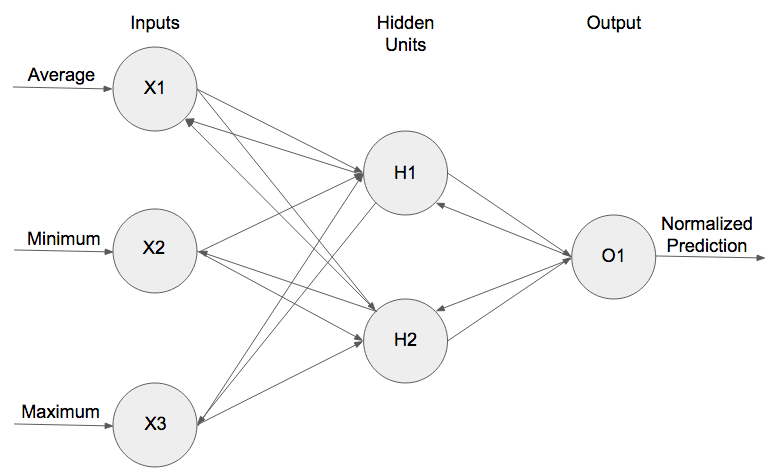
\includegraphics[width=18cm, height=12cm]{bpn}
\caption{Backpropagation Network Architecture}
\end{figure}

It is important to note that this is a \textbf{layered network} in which all hidden units are deeply connected with both the output unit and the input units. 

\subsection{Demystifying BPN Connections}

One common mistake when building neural networks is to get as much data as possible and throw it at the network and expect it to produce good results. In this architecture, we have a deeply connected network because there seems to be a correlation between average, minimum and maximum prices - whereas there might not be a correlation between volume, volatility and earnings. In the case where these factors are to be used, we must be careful not to inner-connect hidden units and input units which have no direct correlation and as such it has led to me choosing this simplified model. For more in-depth networks, the number of hidden units would be tweaked as well as the inputs while varying the connections in order to determine the optimal layout.
Moreover, it is more important to build a base model which can easily be tested first and then improve upon it later with new inputs and different architectures then to throw all existing data at a deeply connected network - which will also help to reduce \textbf{false positives}. 

\section{Training methodology}

As we have discussed in section 1.1, we now have a proper representation of our training set through transforming the moving window time series data generated by \textbf{GOOG} stock closing prices. We train the BPN as the algorithm normally progresses until it can properly approximate all of the expected training outputs. The final source code presents the patterns in order, as experimenting with randomly selecting training vectors did not have much of an improvement over sequential training.

\subsection{Activation Function}

As we have learned in class, the sigmoid function won't suffice in cases where we need to scale data within certain ranges. As such, I've decided to use the \textbf{hyperbolic tan} function as the activation function for the BPN, as it approximates the ramp function for different values of $x$. 

\subsection{Output}

The final output of the neural network will be a normalized predicted value which we then denormalize afterwards. A table will be shown as well as a plot of the actual closing stock price versus predicted closing stock price in the Results section.

\subsection{Testing methodology}

As mentioned earlier, it is better to build a network which can be trained and tested easily. One way to test our network is to take the last two months of closing prices for our stock in question \textbf{GOOG} and partition it with 6 weeks being used for training, and the last 2 weeks for testing. During the testing phase, we build sliding window averages, minimums and maximums of the closing prices during the last 2 weeks, feed it into the network and then check the prediction. By doing this, we can appropriately scale our network by observing it's performance - predicting values days in advance will actually be difficult to test in the real world due to having to wait for these values to be released and then correlated. 

\section{Results}

With all of the technical jargon out of the way, let's take a look at the results.

\begin{figure}[h!]
\centering
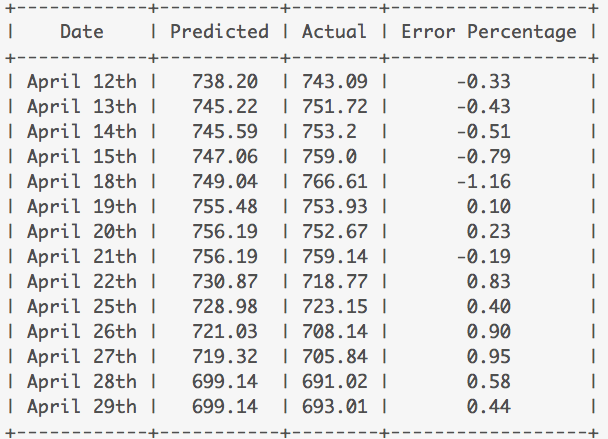
\includegraphics[width=10cm, height=7cm]{market_results}
\caption{BPN Predictions across the last 2 weeks}
\end{figure} 

Not surprisingly, the BPN does not accurately predict the prices. It often underestimates the values, but it does come within a respectable margin of error given the minimal inputs and architecture trickery. Below is a plot of the results:

\begin{figure}[h]
\centering
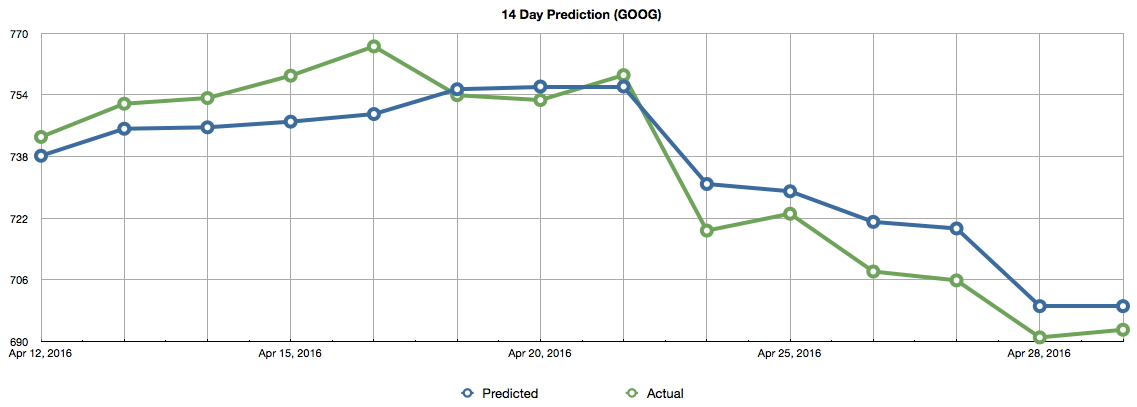
\includegraphics[width=17cm, height=10cm]{plot}
\caption{Line Plot of Predicted vs. Actual Closing Stock Prices}
\end{figure}

\section{Improvements}

As mentioned in section 2.1, introducing new inputs such as stock volatility, volume sold and company earnings could be beneficial inputs if fed in and interconnected correctly. Another interesting input would be a sentiment analysis with regards to the company (Google, in this case) - where various articles published about the company can be analyzed using a tool such as IBM Watson (they have a publicly available API through IBM Bluemix) in order to determine the overall trend towards the company. Naturally, a company with more positive sentiment analysis would correlate to an improvement in stock (at least, it is a reasonable assumption). These features would be great for a thesis project or in the real-world, along with looking into \textbf{deep learning} for stock market predictions. 

\section{Conclusion}

Overall, this project was a blast to work on. It brought me back to my years of doing machine learning - and painfully understanding all of the linear algebra that goes into it. In the past I've used powerful tools such as Theanonets (a Python computing library with powerful matrix operators and neural network functions) and SciKit Learn (another Python library full of neural network tools and functions), but this time I decided to build the network from scratch. In the process, I've learned how to build matrices of the proper shape, how to update the appropriate weights through backpropagation and ultimately learned how to tackle a topic in an unfamiliar field (financial). While my understanding of neural networks is still novice at best, this project was a great eye-opener to all of the tiny details that go into designing these applications - especially when neural networks appear as black boxes that compute magical functions and can only be improved by getting under the hood.

\section{Source Code}

The entirety of the source code for this project may be found below.

\begin{lstlisting}
import math
from numpy import zeros
from numpy import random
from prettytable import PrettyTable

def sigmoid(x):
  return math.tanh(x)

def deltaSigmoid(y):
  return 1.0 - y ** 2

class network:
  def __init__(self, inputs, hidden, outputs):
    # Initialize inputs as well as bias
    self.inputs = inputs + 1

    # Initialize hidden units
    self.hidden = hidden

    # Initialize output units
    self.outputs = outputs

    # Initialize activation for input nodes
    self.input_activations = [1.0] * self.inputs

    # Initialize activation for hidden units
    self.hidden_activations = [1.0] * self.hidden

    # Initialize activation for output units
    self.outputs_activations = [1.0] * self.outputs
    
    # Initialize weight matrix between inputs and hidden units
    self.input_weights = random.rand(self.inputs, self.hidden)

    # Initialize weight matrix between hidden units and outputs
    self.output_weights = random.rand(self.hidden, self.outputs)

    # Learning rate alpha
    self.alpha = 0.5

    # Iterations to train network for
    self.iterations = 1000

  def update(self, inputs):
    # Compute activation for all inputs except bias
    for input in range(self.inputs - 1):
      self.input_activations[input] = inputs[input]

    # Compute activation for all hidden units
    for hidden in range(self.hidden):
      sum = 0.0
      for input in range(self.inputs):
          sum += self.input_activations[input] * self.input_weights[input][hidden]
      self.hidden_activations[hidden] = sigmoid(sum)

    # Compute activation for all output units
    for output in range(self.outputs):
      sum = 0.0
      for hidden in range(self.hidden):
        sum += self.hidden_activations[hidden] * self.output_weights[hidden][output]
      self.outputs_activations[output] = sigmoid(sum)
    return self.outputs_activations

  def backpropagate(self, targets):
    # Compute error at output units
    output_deltas = [0.0] * self.outputs
    for output in range(self.outputs):
      error = targets[output] - self.outputs_activations[output]
      output_deltas[output] = deltaSigmoid(self.outputs_activations[output]) * error

    # Compute error at hidden units
    hidden_deltas = [0.0] * self.hidden
    for hidden in range(self.hidden):
      error = 0.0
      for output in range(self.outputs):
        error += output_deltas[output] * self.output_weights[hidden][output]
      hidden_deltas[hidden] = deltaSigmoid(self.hidden_activations[hidden]) * error

    # Update output unit weights
    for hidden in range(self.hidden):
      for output in range(self.outputs):
        update = output_deltas[output] * self.hidden_activations[hidden]
        self.output_weights[hidden][output] = self.output_weights[hidden][output] 
                                              + self.alpha * update

    # Update input unit weights
    for input in range(self.inputs):
      for hidden in range(self.hidden):
        update = hidden_deltas[hidden] * self.input_activations[input]
        self.input_weights[input][hidden] = self.input_weights[input][hidden] 
                                            + self.alpha * update

    # Compute total error
    error = 0.0
    for target in range(len(targets)):
      error += 0.5 * (targets[target] - self.outputs_activations[target]) ** 2
    return error

  def test(self, pattern):
    # for pattern in patterns:
    print(pattern, '->', self.update(pattern))
    return self.update(pattern)[0]

  def train(self, patterns):
    for iteration in range(self.iterations):
      error = 0.0
      for pattern in patterns:
        inputs = pattern[0]
        targets = pattern[1]
        self.update(inputs)
        error += self.backpropagate(targets)
      if iteration % 100 == 0:
        print('error %-.5f' % error)

def average(data):
  sum = 0.0
  for datum in data:
    sum += datum
  return sum / len(data)

def maximum(data):
  return max(data)

def minimum(data):
  return min(data)

def normalize(price, minimum, maximum):
  return ((2 * price - (maximum + minimum)) / (maximum - minimum))

def denormalize(normalized, minimum, maximum):
  return (((normalized * (maximum-minimum)) / 2) + (maximum + minimum)) / 2

def slidingWindow(data):
  windows = []
  beginning = 0
  end = 5
  i = 0
  while i < 20:
    windows.append(data[beginning:end])
    beginning += 1
    end += 1
    i += 1
  return windows

def run():
  # Closing prices from March 8thth -> April 11th
  dataset = [688.59, 698.47, 708.12, 720.00, 726.81, 726.92, 726.37, 736.45, 741.86, 
    736.50, 737.46, 742.36, 732.01, 736.79, 734.59, 750.10, 
    749.25, 738.60, 750.06, 738.00, 735.77, 745.37, 743.97, 743.02]

  # Compute 5-day sliding windows
  windows = slidingWindow(dataset)

  # Compute the average, minimum, maximum and normalized prices from windows
  computed_data = []
  for window in windows:
    # Prepare [average, minimum, maximum]
    data = []
    ave = average(window)
    min = minimum(window)
    max = maximum(window)
    data.append(ave)
    data.append(min)
    data.append(max)
    computed_data.append(data)

    # Prepare normalized closing value
    closing = []
    closing.append(normalize(window[0], min, max))
    computed_data.append(closing)
  training_data = [computed_data]

  # Create network architecture consisting of 3 input nodes, 2 hidden units, and 1 output unit
  n = network(3, 2, 1)

  # Train the network
  n.train(training_data)

  # Prediction Data (April 12th -> 29th)
  prediction_dataset = [743.09, 751.72, 753.20, 759.00, 766.61, 753.93, 
    752.67, 759.14, 718.77, 723.15, 708.14, 705.84, 691.02, 693.01]

  # Create 5-day sliding windows for prediction data
  complete_dataset = dataset + prediction_dataset

  prediction_windows = []
  for prediction in prediction_dataset:
    location = complete_dataset.index(prediction)
    prediction_windows.append(complete_dataset[location - 4: location + 1])
  
  prediction_data = []
  predictions = []
  # Compute prediction windows in the form of [average, minimum, maximum]
  for window in prediction_windows:
    data = []
    ave = average(window)
    min = minimum(window)
    max = maximum(window)
    data.append(ave)
    data.append(min)
    data.append(max)
    prediction_data.append(data)

  # Test the network
  for i in xrange(len(prediction_data)):
    value = n.test(prediction_data[i])
    predictions.append(denormalize(value, prediction_data[i][1], prediction_data[i][2]))

run()
\end{lstlisting}

\begin{thebibliography}{9}
\bibitem{latexcompanion} 
Yahoo!
\textit{Yahoo! Finance API}. 
http://finance.yahoo.com/q/hp?s=GOOG
 
\bibitem{einstein} 
Jaydip Sen, Tamal Datta Chaudhuri.
\textit{Decomposition of Time Series Data of Stock Markets and its
Implications for Prediction � An Application for the Indian Auto}.
 
 
\bibitem{einstein} 
S. C. Nayak, B. B. Misra, H. S. Behera
\textit{Impact of Data Normalization on Stock Index
Forecasting}. 
International Journal of Computer Information Systems and Industrial Management Applications, 2014.

\bibitem{einstein} 
Abhishek Kar. 
\textit{Stock Prediction using Artificial Neural Networks} (Y8021).

\bibitem{einstein} 
Steven Miller. 
\textit{Mind: How to Build a Neural Network (Part One)}
http://stevenmiller888.github.io/mind-how-to-build-a-neural-network/

\bibitem{einstein} 
Steven Miller. 
\textit{Mind: How to Build a Neural Network (Part Two)}
http://stevenmiller888.github.io/mind-how-to-build-a-neural-network-part-2/

\end{thebibliography}

\end{document}
